%# -*- coding: utf-8-unix -*-
%%==================================================
%%%%%%%%%%%%%%%%%%%%%%%%%%%%%%%%%%%%%%%%%
\chapter{不确定性推理}
%%%%%%%%%%%%%%%%%%%%%%%%%%%%%%%%%%%%
\begin{tcolorbox}[colback=white!50,colframe=orange!50,title=不精确性推理方法]
\begin{center}
现实世界中的大多数问题是不精确、非完备的.对于这些问题, 若采用前面所讨论的精确性推理方法显然是无法解决的.
为此, 人工智能需要研究不精确性的推理方法, 以满足客观问题的需求.
\hfill
\end{center}
\end{tcolorbox}
%%%%%%%%%%%%%%%%%%%%%%%%%%%%%%%%%%%%%%%%%%
\begin{figure}[H]
\centering

\includegraphics[width=0.84\textwidth]{KRR20191218002.jpg}
\label{KRR20191218002}
\end{figure}
%%%%%%%%%%%%%%%%%%%%%%%%%%%%%%%%%%
%%%%%%%%%%%%%%%%%%%%%%%%%%%%%%%%%%%%%%%%%
\section{不确定性推理的含义}
%%%%%%%%%%%%%%%%%%%%%%%%%%%%%%%%%%%%%%%%%
\paragraph{什么是不确定性推理}
\begin{itemize}
\item 不确定性推理泛指除精确推理以外的其它各种推理问题.包括不完备、不精确知识的推理, 模糊知识的推理, 非单调性推理等.
\item 不确定性推理过程实际上是一种从不确定的初始证据出发, 通过运用不确定性知识, 最终推出具有不确定性但却又是合理或基本合理结论的思维过程.
\end{itemize}
%%%%%%%%%%%%%%%%%%%%%%%%%%%%%%%%%%%%%%%%%
\paragraph{为什么要采用不确定性推理}
\begin{itemize}
\item  所需知识不完备.
\item  不精确所需知识描述模糊.
\item  多种原因导致同一结论.
\item  问题的背景知识不足.
\item  解题方案不唯一.
\end{itemize}
%%%%%%%%%%%%%%%%%%%%%%%%%%%%%%%%%%%%%%%%%
\section{不确定性推理的基本问题 }\label{AI32C6Sec6.2}
%%%%%%%%%%%%%%%%%%%%%%%%%%%%%%%%%%%%%%%%%
\paragraph{不确定性的表示}

(1) 知识的不确定性的表示
\begin{itemize}
\item 考虑因素: 问题的描述能力

      推理中不确定性的计算.

\item 含义: 知识的确定性程度, 或动态强度.
\item 表示: 用概率, [0,1], 0接近于假, 1接近于真. 用可信度, [-1,1], 大于0接近于真,小于0接近于假.
\end{itemize}

(2) 证据的非精确性表示

    证据来源: 初始证据, 中间结论.
    表示: 用概率或可信度.
\begin{itemize}
\item 含义: 不确定的前提条件与不确定的事实匹配.
\item 问题: 前提是不确定的, 事实也是不确定的.
\item 方法: 设计一个计算相似程度的算法, 给出相似的限度.
\item 标志: 相似度落在规定限度内为匹配, 否则为不匹配.
\item 含义: 知识的前提条件是多个证据的组合.
\item 方法: 最大最小方法, 如合取取最小、析取取最大.

    概率方法, 按概率
\end{itemize}

4. 非精确性的更新

    主要问题

    \ding{172} 如何用证据的不确定性去更新结论的不确定性.

    \ding{173} 如何在推理中把初始证据的不确定性传递给最终结论.

    解决方法

    对\ding{172} 不同推理方法的解决方法不同.

    对\ding{173} 不同推理方法的解决方法基本相同, 即把当 前结论及其不确定性作为新的结论放入综合数据库, 依次 传递, 直到得出最终结论.

5. 非精确性结论的合成

    含义: 多个不同知识推出同一结论, 且不确定性程度不同.

    方法: 视不同推理方法而定.
%%%%%%%%%%%%%%%%%%%%%%%%%%%%%%%%%%%%%%%%%%
\begin{figure}[H]
\centering
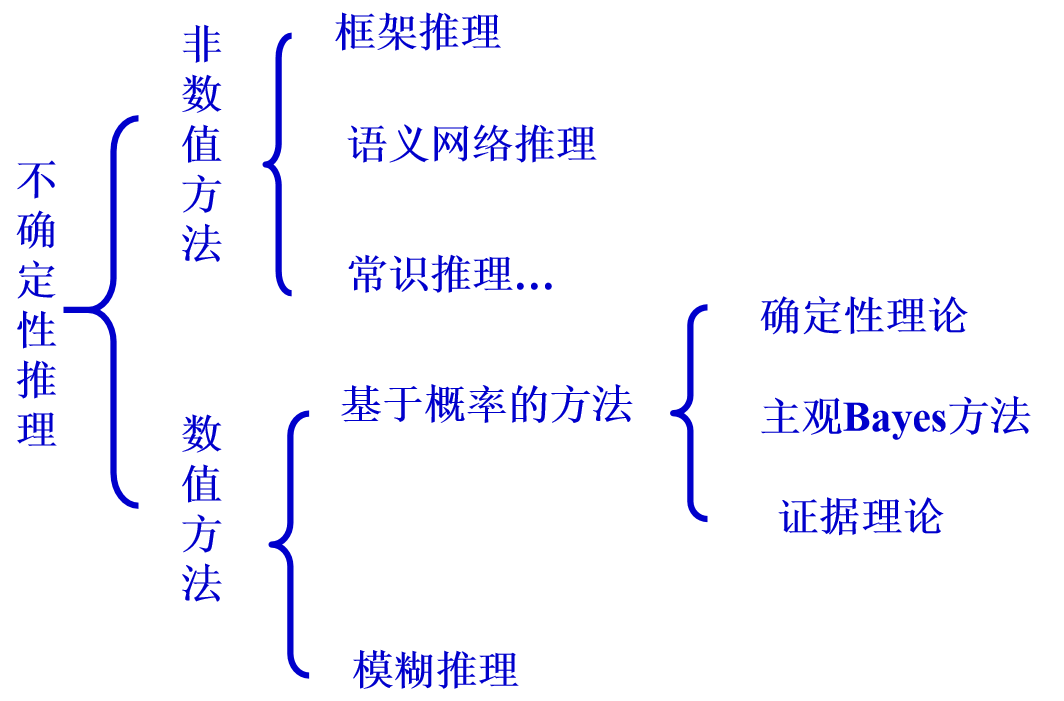
\includegraphics[width=0.6\textwidth]{AI32C42019112618.PNG}
\caption{不确定方法}
\label{AI32fig2618}
\end{figure}
%%%%%%%%%%%%%%%%%%%%%%%%%%%%%%%%%%%%%%%%%%
%%%%%%%%%%%%%%%%%%%%%%%%%%%%%%%%%%%%%%%%%
\section{不确定性推理的概率论基础}
在概率论中, 把试验中每一个可能出现的结果称为试验的一个样本点, 由全体样本点构成的集合称为样本空间.

表示:通常用$D$表示样本空间, $d$表示样本点.

\begin{example}
  在掷币试验中, 若用$d_1$表示硬币的正面向上, 用$d_2$表示硬币的反面向上, 则该试验的样本空间为: $D=\{d_1, d_2\}$.
\end{example}

概念:由样本点构成的集合称为随机事件.

\begin{example}
  在掷币试验中, 若用$A$表示硬币正面向上这一事件, 则有$A=\{d_1\}$.
\end{example}

概率运算
\begin{itemize}
\item 并事件: 事件$A$与事件$B$至少有一个发生, 记为$A\cup B$.

\item 交事件: 事件$A$与事件$B$同时发生, 记为$A\cap B$.

\item 互逆事件
\item 事件$A$与$B$之间满足“$A\cap B=\emptyset,  A\cup B=D$”.
\end{itemize}

%%%%%%%%%%%%%%%%%%%%%%%%%%%%%%%%%%
\begin{mydef}{频率的概念}{1}
统计概率是通过某一事件出现的频率定义的. 频率定义为
\begin{align}
  f_n(A)=m/n
\end{align}
式中, $A$所讨论的事件, $n$是试验的总次数, $m$是实验中$A$发生的次数.
\end{mydef}

%%%%%%%%%%%%%%%%%%%%%%%%%%%%%%%%%%
\begin{mydef}{概率的统计定义}{1}
在同一组条件下所进行大量重复试验时, 如果事件A出现的频率总是在区间$[0, 1]$上的一个确定常数$p$附近摆动, 并且稳定于$p$, 则称$p$为事件$A$的统计概率. 即
\begin{align}
  P(A)=p.
\end{align}
\end{mydef}
%%%%%%%%%%%%%%%%%%%%%%%%%%%%%%%%%%%
\begin{example}
在掷币试验中, 当掷币次数足够多时有
\begin{align}
  f_n(\textup{正面向上})=0.5.
\end{align}
则称正面向上的概率为0.5, 即
\begin{align}
  P(\textup{正面向上})=0.5.
\end{align}
\end{example}
%%%%%%%%%%%%%%%%%%%%%%%%%%%%%%%%%%
\begin{mydef}{统计概率的性质}{1}
(1)对任一事件$A$, 有$ 0\leq P(A)\leq 1$.

    (2)必然事件$D$的概率$P(D)=1$, 不可能事件Φ的概率$P(\emptyset)=0$.

    (3)对任一事件A, 有$P(\neg A)=1-P(A)$.

    (4)设事件$A_1, A_2 ,\cdots , A_k (k\leq n)$是两两互不相容的事件, 即有 $A_i\cap A_j=Φ (i\neq j)$, 则

    (5)设$A, B$是两个事件, 则$P(A\cup B)=P(A)+P(B)-P(A\cap B)$.
\end{mydef}
%%%%%%%%%%%%%%%%%%%%%%%%%%%%%%%%%%
\begin{mydef}{条件概率}{1}
设$A$与$B$是两个随机事件, $P(B)>0$, 则称:
\begin{align}
  P(A|B)=P(A\cap B)/P(B)
\end{align}
为在事件$B$发生的条件下事件$A$的条件概率 .
\end{mydef}
%%%%%%%%%%%%%%%%%%%%%%%%%%%%%%%%%%
\begin{example}
设样本空间$D$是扑克牌中的54张牌, 即D=\{红桃A, 方块A, 黑桃A, 梅花A, 红桃2, 方块2, $\cdots$, 小王, 大王\}, 且有以下两个事件 $A=\textup{\{取花脸牌\}},B=\textup{\{取红桃牌\}}$,
求在事件$B$发生的条件下事件A发生的概率$P(A|B)$.
\end{example}

\begin{result}
由于事件$B$已经发生, 因此以下事件\{取到红桃$A$; 取到红桃2; 取到红桃3; $\cdots$; 取到红桃$K$\}中必有一个出现.

而对事件$A$, 在事件$B$发生的前提下, 只有以下事件\{取到红桃$J$; 取到红桃$Q$; 取到红桃$K$中的一个\}发生时事件$A$才能发生.

因此, 在事件$B$发生的条件下事件$A$发生的概率是3/13.
\end{result}
%%%%%%%%%%%%%%%%%%%%%%%%%%%%%%%%%%
\begin{mythm}{全概率公式}{1}
设事件$A_1,A_2,\cdots,A_n$满足:

    (1)任意两个事件都互不相容, 即当$i\neq j$时, 有$A_i\cap A_j=\emptyset, (i=1,2,\cdots ,n_j=1,2,\cdots ,n)$;

    (2) $P(A_i)>0 (i=1, 2, \cdots, n)$;

    (3) $D=\bigcup_{n=1}^{n} A_{n}$, 则对任何事件$B$由下式成立:
\begin{align}
  P(B)=\sum_{i=1}^{n} P\left(A_{i}\right) \times P\left(B | A_{i}\right).
\end{align}
该公式称为全概率公式, 它提供了一种计算$P(B)$的方法.
\end{mythm}
%%%%%%%%%%%%%%%%%%%%%%%%%%%%%%%%%%
\begin{mythm}{Bayes定理}{1}
设事件$A_1,A_2,\cdots,A_n$满足定理6.1规定的条件, 则对任何事件$B$有下式成立:
\begin{align}
P\left(A_{i} | B\right)=\frac{P\left(A_{i}\right) \times P\left(B / A_{i}\right)}{\sum_{j=1}^{n} P\left(A_{j}\right) \times P\left(B / A_{j}\right)}, i=1,2, \cdots, n.
\end{align}
该定理称为\textbf{Bayes定理}, 上式称为Bayes公式. 其中$P(A_i)$是事件$A_i$的先验概率, $P(B|A_i)$是在事件$A_i$发生条件下事件$B$的条件概率; $P(A_i|B)$是在事件$B$发生条件下事件$A_i$的条件概率.
\end{mythm}

如果把全概率公式代入Bayes公式, 则有:
\begin{align}
  P\left(A_{i} | B\right)=\frac{P(A) \times P\left(B | A_{i}\right)}{P(B)}, i=1,2, \cdots, n,
\end{align}
即
\begin{align}
  P\left(A_{i} | B\right) \times P(B)=P\left(B_{i} | A\right) \times P\left(A_{i}\right), i=1,2, \ldots, n.
\end{align}
这是Bayes公式的另一种形式.

Bayes定理给出了用逆概率$P(B|A_i)$求原概率$P(A_i|B)$的方法.
%%%%%%%%%%%%%%%%%%%%%%%%%%%%%%%%%%%%%%%%%
\subsection{可信度的概念}
可信度是指人们根据以往经验对某个事物或现象为真的程度的一个判断, 或者说是人们对某个事物或现象为真的相信程度.
\begin{example}
  沈强昨天没来上课, 理由是头疼. 就此理由, 只有以下两种可能: 一是真的头疼了, 理由为真; 二是没有头疼, 理由为假. 但就听话人而言, 因不能确切知道, 就只能某种程度上相信, 即可信度.
\end{example}

可信度具有一定的主观性, 较难把握.但对某一特定领域, 让该领域专家给出可信度还是可行的.
%%%%%%%%%%%%%%%%%%%%%%%%%%%%%%%%%%%%%%%%%
\subsection{CF模型}

1. 知识不确定性的表示

表示形式:

在C-F模型中, 知识是用产生式规则表示的, 其一般形式为:
\begin{center}
  IF\,\,   E\,\,    THEN\,\,  H\,\, (CF($H, E$)),
\end{center}
其中, $E$是知识的前提条件; $H$是知识的结论; CF($H, E$)是知识的可信度.
\begin{remark}
(1) $E$可以是单一条件, 也可以是复合条件.
    \begin{example}
        \begin{center}
          $E$=($E_1$  OR  $E_2$)  AND  $E_3$  AND  $E_4$.
        \end{center}
    \end{example}

(2) $H$可以是单一结论, 也可以是多个结论.

(3) CF是知识的静态强度, CF($H, E$)的取值为$[-1, 1]$, 表示当$E$为真时, 证据对$H$的支持程度, 其值越大, 支持程度越大.
\end{remark}

%%%%%%%%%%%%%%%%%%%%%%%%%%%%%%%%%%%%%%%%%%%%%%%%%%%%%%%
\begin{example}
\begin{center}
      IF   发烧    AND  流鼻涕   THEN   感冒   (0.8),
\end{center}
表示当某人确实有“发烧”及“流鼻涕”症状时, 则有80\%的把握是患了感冒.
\end{example}
%%%%%%%%%%%%%%%%%%%%%%%%%%%%%%%%%%%%%%%%%%%%%%%%%%%%%%%
\subsection{可信度的定义与性质}
%%%%%%%%%%%%%%%%%%%%%%%%%%%%%%
\paragraph{可信度的定义}
在$CF$模型中, 把$CF(H, E)$定义为
          $$CF(H, E)=MB(H, E)-MD(H, E),$$
式中$MB$称为信任增长度, $MB(H, E)$定义为
\begin{align}
  MB(H, E)=\left\{\begin{array}{ll}{1,} & \textup{若} P(H)=1 \\
  {\frac{\max \{P(H | E), P(H)\}-P(H)}{1-P(H)},} & \textup{否则}
  \end{array}\right.,
\end{align}
$MD$称为不信任增长度, $MB(H, E)$定义为
\begin{align}
  MD(H, E)=\left\{\begin{array}{ll}{1,} &  \textup{若} P(H)=0 \\
  {\frac{\min \{P(H | E), P(E)\}-P(H)}{-P(H)},} &\textup{否则}\end{array}\right.
\end{align}
%%%%%%%%%%%%%%%%%%%%%%%%%%%%%%
\subparagraph{MB和MD的关系}
\begin{center}
    \ding{172} 当$MB(H, E)>0$时, 有$P(H|E)>P(H)$, 即$E$的出现增加了$H$的概率;

    \ding{173} 当$MD(H, E)>0$时, 有$P(H|E)<P(H)$, 即$E$的出现降低了$H$的概率.
\end{center}

根据前面对$CF(H, E)$可信度 、$MB(H, E)$信任增长度、$MD(H, E)$不信增长度的定义, 可得到$CF(H, E)$的计算公式:
\begin{align}
  C F(H, E)=\left\{\begin{array}{ll}
  {M B(H, E)-0=\frac{P(H | E)-P(H)}{1-P(H)}} & \textup{若}P(H | E)>P(H) \\
  {0} & \textup{若} P(H | E)=P(H) \\
  {0-M D(H, E)=-\frac{P(H)-P(H | E)}{P(H)}} & \textup{若} P(H | E)<P(H)
  \end{array}\right.
\end{align}
分别解释$CF(H,E)>0, CF(H,E)=0, CF(H,E)>0$.
%%%%%%%%%%%%%%%%%%%%%%%%%%%%%%
\subparagraph{可信度的性质}
\begin{itemize}
\item 互斥性

对同一证据, 它不可能既增加对$H$的信任程度, 又同时增加对$H$的不信任程度, 这说明$MB$与$MD$是互斥的.即有如下互斥性:

   $\bullet$当$MB(H, E)>0时, MD(H, E)=0$;

   $\bullet$当$MD(H, E)>0时, MB(H, E)=0$.
\item 值域
\item 典型值

    当$CF(H,E)=1$时, 有$P(H/E)=1$, 它说明由于$E$所对应证据的出现使$H$为真.此时, $MB(H, E)=1, MD(H, E)=0$.

    当$CF(H,E)= -1$时, 有$P(H/E)=0$, 说明由于$E$所对应证据的出现使$H$为假.此时, $MB(H, E)=0, MD(H,E)=1$.

    当$CF(H,E)= 0$时, 有$MB(H, E)=0$、$MD(H, E)=0$.前者说明$E$所对应证据的出现不证实$H$; 后者说明$E$所对应证据的出现不否认$H$.

\item 典型值对$H$的信任增长度等于对非$H$的不信任增长度.
\end{itemize}

根据$MB$、$MD$的定义及概率的性质有:

\begin{align}
M D(\neg H, E) &=\frac{P(\neg H | E)-P(\neg H)}{-P(\neg H)}=\frac{(1-P(H | E))-(1-P(H))}{-(1-P(H))}\notag \\
&=\frac{-P(H | E)+P(H)}{-(1-P(H))}=\frac{-(P(H | E)-P(H))}{-(1-P(H))}\notag\\
&=\frac{P(H | E)-P(H)}{1-P(H)}=MB(H, E). \textup{信任增长度}
\end{align}

再根据CF的定义和MB、MD的互斥性有
\begin{align*}
CF(H,E)+CF(\neg H,E)
              &=(MB(H,E)-MD(H,E))+(MB(\neg H,E)-MD(\neg H,E))\\
              &=(MB(H,E)-0)+(0-MD(\neg H,E))                                     \textup{(由互斥性)}\\
              &=MB(H,E)-MD(\neg H,E)=0.
\end{align*}
它说明

        (1)对$H$的信任增长度等于对非$H$的不信任增长度.

        (2)对$H$的可信度与非$H$的可信度之和等于0.

        (3)可信度不是概率, 不满足
\begin{align*}
  P(H)+P(\neg H)=1, 0\leq P(H), P(\neg H)\leq 1.
\end{align*}

(5)对同一前提$E$, 若支持若干个不同的结论$H_i\,(i=1,2,\cdots,n)$, 则
\begin{align*}
  \sum_{i=1}^{n} C F\left(H_{i}, E\right) \leq 1,
\end{align*}
因此, 如果发现专家给出的知识有如下情况
\begin{align*}
  CF(H_1, E)=0.7,  CF(H_2, E)=0.4,
\end{align*}
则因$0.7+0.4=1.1>1$为非法, 应进行调整或规范化.
%%%%%%%%%%%%%%%%%%%%%%%%%%%%%%%%%%%%%%%%%
\section{证据理论}
\subsection{证据不确定性的表示}
%%%%%%%%%%%%%%%%%%%%%%%%%%
\paragraph{不确定性的表示}
证据的不确定性也是用可信度来表示的, 其取值范围也为$[-1,1]$. 
\begin{itemize}
\item 若$E$为初始证据, 其值由用户给出.
\item 若$E$为中间结论, 其值可通过计算得到.
\end{itemize}
%%%%%%%%%%%%%%%%%%%%%%%%%%
\paragraph{不确定性的含义}
对$E$, 其可信度$CF(E)$的含义如下:
\begin{center}
\begin{itemize}
\item $CF(E)=1$, 证据$E$肯定它为真;
\item $CF(E)=-1$, 证据$E$肯定它为假;
\item $CF(E)=0$, 对证据$E$一无所知;
\item $0<CF(E)<1$, 证据$E$以CF(E)程度为真;
\item $-1<CF(E)<0$, 证据$E$以CF(E)程度为假.
\end{itemize}
\end{center}
%%%%%%%%%%%%%%%%%%%%%%%%%%
\paragraph{ 否定证据不确定性的计算}
\begin{align}
  CF(\neg E)=-CF(E).
\end{align}
%%%%%%%%%%%%%%%%%%%%%%%%%%
\paragraph{组合证据不确定性的计算}
对证据的组合形式可分为“合取”与“析取”两种基本情况.
\begin{itemize}
\item 合取

    当组合证据是多个单一证据的组合时, 即 $E=E_1\,\,  AND\,\,    E_2\,\,    AND \,\,   \cdots\,\,     AND \,\,   E_n$时, 若已知$CF(E_1), CF(E_2), \cdots , CF(E_n)$, 则
\begin{align}
  CF(E)=\min\{CF(E_1), CF(E_2), \cdots  ,CF(E_n)\}.
\end{align}
\item 析取

 当组合证据是多个单一证据的析取时, 即$E=E_1\,\,  \textup{OR}\,\,  E_2 \,\, \textup{OR}\,\,  \cdots \,\,  \textup{OR}\,\, E_n$时, 若已知$CF(E_1), CF(E_2), \cdots , CF(E_n)$, 则
\begin{align}
  CF(E)=\max\{CF(E_1), CF(E_2), \cdots  ,CF(E_n)\}.
\end{align}
\end{itemize}

%%%%%%%%%%%%%%%%%%%%%%%%%%%%%%%%%%%%%%%%%%%%%
\subsection{不确定性的更新}
 CF模型中的不确定性推理实际上是从不确定的初始证据出发, 不断运用相关的不确性知识, 逐步推出最终结论和该结论可信度的过程.而每一次运用不确定性知识, 都需要由证据的不确定性和知识的不确定性去计算结论的不确定性.

不确定性的更新公式
\begin{align}
  CF(H)=CF(H, E)\times \max\{0, CF(E)\}.
\end{align}
    若$CF(E)<0$, 则
\begin{align}
  CF(H)=0,
\end{align}
即该模型没考虑$E$为假对$H$的影响.

若$CF(E)=1$, 则
\begin{align}
  CF(H)=CF(H,E),
\end{align}
即规则强度$CF(H,E)$实际上是在$E$为真时, $H$的可信度.
%%%%%%%%%%%%%%%%%%%%%%%%%%%%%%%%%%%
\subsection{结论不确定性的合成}
当有多条知识支持同一个结论, 且这些知识的前提相互独立, 结论的可信度又不相同时, 可利用不确定性的合成算法求出结论的综合可信度.
    设有知识:
\begin{align}
  &\textup{IF}\,\,    E_1\,\,     \textup{THEN} \,\,    H(CF(H, E_1));\\
  &\textup{IF}\,\,    E_2 \,\,    \textup{THEN} \,\,    H(CF(H, E_2)).
\end{align}
则结论$H$的综合可信度可分以下两步计算:

(1) 分别对每条知识求出其$CF(H)$. 即
\begin{align}
  &CF_1(H)=CF(H, E_1) \times\max\{0, CF(E_1)\};\\
  &CF_2(H)=CF(H, E_2)\times\max\{0, CF(E_2)\}.
\end{align}

(2) 用如下公式求$E_1$与$E_2$对$H$的综合可信度
\begin{align}
 CF(H)=\left\{
 \begin{array}{llr}
  {C F_{1}(H)+C F_{2}(H)-C F_{1}(H) \times C F_{2}(H)}  & \textup{若} CF_{1}(H) \geq 0 \\
  {} & {\textup{且} C F_{2}(H) \geq 0} \\
  {C F_{1}(H)+C F_{2}(H)+C H_{1}(H) \times CF_{2}(H)} & \textup{若} CF_{1}(H)<0 \\
   {C F_{1}(H)+C F_{2}(H)}                            & \textup{若} CF(H)< 0\\
    \frac{C F_{1}(H)+C F_{2}(H)}{1-\min \left\{C F_{1}(H),\left|CF_{2}(H)\right|\right\}} &\textup{且} CF_{2}(H) \vec{F}
    \end{array}
  \right..
\end{align}

\begin{example}
设有如下一组知识:
\begin{Verbatim}
     $r_1$: IF  E1  THEN  H(0.9);
     $r_2$: IF  E2  THEN  H(0.6);
     $r_3$: IF  E3  THEN  H(-0.5);
     $r_4$: IF  E4  AND  ( E5  OR  E6)  THEN  E1(0.8).
\end{Verbatim}
已知: $CF(E_2)=0.8, CF(E_3)=0.6, CF(E_4)=0.5, CF(E_5)=0.6, CF(E_6)=0.8$, 求$CF(H)=?$
\end{example}
%%%%%%%%%%%%%%%%%%%%%%%%%%%%%%%%%
\begin{result}
由$r_4$得到:
\begin{align*}
    CF(E_1)&=0.8\times \max\{ 0, CF(E_4  AND  (E_5  OR   E_6)) \}\\
          &=0.8\times \max\{ 0, \min\{CF(E_4),  CF(E_5  OR   E_6)\} \}\\
          &=0.8\times \max\{ 0, \min\{CF(E_4),  \max\{CF(E_5),  CF(E_6)\}\} \}\\
          &=0.8\times \max\{ 0, \min\{CF(E_4),  \max\{0.6,  0.8\}\} \}\\
          &=0.8\times \max\{ 0, \min\{0.5,  0.8\} \}\\
          &=0.8\times \max\{ 0,  0.5 \} = 0.4.
\end{align*}
\end{result}
由$r_1$得到:
\begin{align*}
CF_1(H)&=CF(H, E_1)\times \max\{0,  CF(E_1)\}=0.9\times \max\{0,  0.4\} = 0.36.
\end{align*}
    由$r_2$得到:
\begin{align*}
CF_2(H)&=CF(H, E_2)\times \max\{0,  CF(E_2)\}=0.6\times \max\{0,  0.8\} = 0.48.
\end{align*}
由$r_3$得到:
\begin{align*}
CF_3(H)&=CF(H, E_3)\times \max\{0,  CF(E_3)\}=-0.5\times \max\{0,  0.6\} = -0.3.
\end{align*}

根据结论不精确性的合成算法, $CF_1(H)$和$CF_2(H)$同号, 有:
\begin{align}
  \begin{aligned}
  C F_{1,2}(H) &=C F_{1}(H)+C F_{2}(H)-C F_{1}(H) \times C F_{2}(H) \\
  &=0.36+0.48-0.36 \times 0.48 \\
  &=0.84-0.17=0.67.
  \end{aligned}
\end{align}

$CF_{12}(H)$和$CF_3(H)$异号, 有:
\begin{align}
  \begin{aligned}
  C F_{1,2,3}(H) &=\frac{C F_{1,2}(H)+C F_{3}(H)}{1-\min \left\{\left\langle C F_{1,2}(H)|,| C F_{3}(H)\right|\right\}} \\
  &=\frac{0.67-0.3}{1-\min\{0.67,0.3\}}=\frac{0.37}{0.7} \\
  &=0.53.
  \end{aligned}
\end{align}
%%%%%%%%%%%%%%%%%%%%%%%%%%%%%%%%%%%%%%%%%
\section{主观Bayes方法}
在主观Bayes方法中, 知识是用产生式表示的, 其形式为:
\begin{align}
   \textup{IF} \,\, E\,\,  \textup{THEN}\,\,  \textup{(LS, LN)} \,\,  H,
\end{align}
其中, (LS, LN)用来表示该知识的知识强度, LS(充分性度量)和LN(必要性度量)的表示形式分别为:
\begin{align}
\begin{aligned}
LS &=\frac{P(E | H)}{P(E | \neg H)}; \\
LN &=\frac{P(\neg E | H)}{P(\neg E | \neg H)}=\frac{1-P(E | H)}{1-P(E | \neg H)}.
\end{aligned}
\end{align}
下面进一步讨论LS和LN的含义.由本章第\ref{AI32C6Sec6.2}节的Bayes公式可知:
\begin{align}\label{AI32C6eq6.2}
  \begin{aligned}
  P(H | E) &=\frac{P(E | H) \times P(H)}{P(E)} \\ P(\neg H | E) &=\frac{P(E | \neg H) \times P(\neg H)}{P(E)}.
  \end{aligned}
\end{align}

两式相除得:
\begin{align}
  \frac{P(H | E)}{P(\neg H | E)}=\frac{P(E | H)}{P(E | \neg H)} \times \frac{P(H)}{P(\neg H)}.
\end{align}
为讨论方便, 下面引入几率函数的概念
 %%%%%%%%%%%%%%%%%%%%%%%%%%%%%%%%%
\begin{mydef}{几率函数}{1}
\begin{align}
  O(X)=\frac{P(X)}{1-P(X)} P(X)=\frac{P(X)}{P(\neg X)}.
\end{align}
\end{mydef}

可见, $X$的几率等于$X$出现的概率与$X$不出现的概率之比, $P(X)$与$O(X)$的变化一致, 且有:
\begin{align}\label{AI32C6eq6.1}
P(X)=0,&\,O(X)=0;\\
P(X)=1,&\,O(X)=+\infty.
\end{align}
即把取值为$[0,1]$的$P(X)$放大为取值为$[0,+\infty]$的$O(X)$

把\eqref{AI32C6eq6.2}式代入\eqref{AI32C6eq6.1}式有:
\begin{align}
  O(H | E)=\frac{P(E | H)}{P(E | \neg H)} \times O(H).
\end{align}
再把LS代入此式, 可得:
\begin{align}
  Q(H | E)=LS \times QH.
\end{align}

同理可得到关于LN的公式:
\begin{align}
&\frac{P(H|\neg E)}{P(\neg H|\neg E)}=\frac{P(E | H)}{P(\neg E |\neg H)} \times \frac{P(H)}{P(-H)}\label{AI32C6eq6.36} \\
&Q(H| \neg E)=L N \times Q H)\label{AI32C6eq6.37}
\end{align}
式\eqref{AI32C6eq6.36}和\eqref{AI32C6eq6.37}就是修改的Bayes公式.
%%%%%%%%%%%%%%%%%%%%%%%%%%%%%%%%%%%%%%%%%
\section{证据理论}
证据理论是由德普斯特(A. P. Dempster)首先提出, 并有沙佛(G. Shafer)进一步发展起来的用于处理不确定性的一种理论, 也称DS (Dempster-Shafer)理论.它将概率论中的单点赋值扩展为集合赋值, 可以处理由“不知道”所引起的不确定性, 比主观Bayes方法有着更大的灵活性.
%%%%%%%%%%%%%%%%%%%%%%%%%%%%%%%%%%%%%%%%%
\section{DS理论的形式描述}
在DS理论中, 可以分别用信任函数、似然函数及类概率函数来描述知识的精确信任度、不可驳斥信任度及估计信任度.

DS理论处理的是集合上的不确定性问题, 为此需要先建立命题与集合之间的一一对应关系, 以把命题的不确定性问题转化为集合的不确定性问题.

设$\Omega$为样本空间, 且$\Omega$Ω中的每个元素都相互独立, 则由Ω的所有子集构成的幂集记为$2^\Omega$.
当$\Omega$中的元素个数为N时, 则其幂集$2^{\Omega}$的元素个数为$2^N$, 且其中的每一个元素都对应于一个关于$x$取值情况的命题.

\begin{example}
  设$\Omega=\{\textup{红,黄,白}\}$, 求$\Omega$的幂集$2^{\Omega}$.
\end{example}
%%%%%%%%%%%%%%%%%%%%%%%%%%%%%%%%%%%%%%
\begin{result}
$\Omega$的幂集可包括如下子集:
\begin{align}
  &A_0=\emptyset,             A_1=\{\textup{红}\},         A_2=\{\textup{黄}\},         A_3=\{\textup{白}\},\notag\\
  &A_4=\{\textup{红,黄}\},       A_5=\{\textup{红,白}\},     A_6=\{\textup{黄,白}\},     A_7=\{\textup{红,黄,白}\}\notag
\end{align}
其中, $\emptyset$表示空集, 空集也可表示为$\{\}$.上述子集的个数正好是$2^3 =8$.
\end{result}
%%%%%%%%%%%%%%%%%%%%%%%%%%%%%%%%%%%%%%
\begin{example}
设函数$m: 2^{\Omega}\rightarrow [0,1]$, 且满足
\begin{align}
  \begin{array}{l}
  m(\Phi)=0; \\
  \sum_{A \subseteq \Omega} m(A)=1.
  \end{array}
\end{align}
则称$m$是$2^{\Omega}$上的概率分配函数, $m(A)$称为$A$的基本概率数.
\end{example}

%%%%%%%%%%%%%%%%%%%%%%%%%%%%%%%%%%%%%%
\begin{example}
若定义$2^{\Omega}$上的一个基本函数$m$:
\begin{align}
  m(\{\emptyset,\textup{红}\},& \{\textup{黄}\}, \{\textup{白}\}, \{\textup{红, 黄}\}, \{\textup{红, 白}\}, \{\textup{黄, 白}\}, \{\textup{红, 黄, 白}\})\notag\\
              &=(0, 0.3, 0, 0.1, 0.2, 0.2, 0, 0.2).
\end{align}
其中, $(0, 0.3, 0, 0.1, 0.2, 0.2, 0, 0.2)$分别是幂集$2^{\Omega}$中各个子集的基本概率数.
显然$m$满足概率分配函数的定义.
\end{example}
\begin{remark}\textbf{概率分配函数的说明}
(1) 概率分配函数的作用是把$\Omega$的任一子集映射为$[0,1]$上的一个数$m(A)$.
\begin{itemize}
\item 当$A \subset \Omega $, 且$A$由单个元素组成时, 则$m(A)$表示对$A$的精确信任度;
\item 当$A \subset \Omega $、$A\neq \Omega $, 且$A$由多个元素组成时, $m(A)$也表示对A的精确信任度, 但却不知道这部分信任度该分给$A$中哪些元素;
\item 当$A \subseteq\Omega $时, 则$m(A)$也表示不知道该如何分配的部分.
\end{itemize}
\end{remark}
%%%%%%%%%%%%%%%%%%%%%%%%%%%%%%%%%%%%%%%%%%%% 
\begin{example}
对上例所给出的有限集$\Omega$及基本函数$m$, 当
\begin{itemize}
\item $A=$\{红\}时, 有$m(A)=0.3$, 它表示对命题“$x$是红色”的精确信任度为0.3.
\item $B= $\{红, 黄\}时, 有$m(B)=0.2$, 它表示对命题“$x$或者是红色, 或者是黄色”的精确信任度为0.2, 却不知道该把这0.2分给\{红\}还是分给\{黄\}.
\item $C=\Omega =$\{红, 黄, 白\}时, 有$m(\Omega )=0.2$, 表示不知道该对这0.2如何分配, 但知道它不属于{红}, 就一定属于\{黄\}或\{白\} .
\end{itemize}
\end{example}

(2) 概率分配函数不是概率
%%%%%%%%%%%%%%%%%%%%%%%%%%%%%%%%
\begin{example}
在例6.5中, $m$符合概率分配函数的定义, 但
\begin{align}
  m(\{\textup{红}\})+m(\{\textup{黄}\})+m(\{\textup{白}\})=0.3+0+0.1=0.4<1.
\end{align}
\end{example}
因此$m$不是概率测度, 因为概率$P$要求: $P(\{\textup{红}\})+P(\textup{黄})+P(\textup{白})=1$.

%%%%%%%%%%%%%%%%%%%%%%%%%%%%%%%%%
\begin{mydef}{信任函数}{1}
信任函数$Bel: 2^{\Omega}\rightarrow [0,1]$为
\begin{align}
  \operatorname{Bel}(A)=\sum_{B \subseteq A} m(B),
\end{align}
其中, $2^\Omega$是$\Omega$的幂集. $Bel$又称为下限函数, $Bel(A)$表示对$A$的总的信任度.
\end{mydef}
%%%%%%%%%%%%%%%%%%%%%%%%%%%%%%%%%%%%%%%%%%%%
\begin{example}
对例6.5有
\begin{align}
  &Bel(\{\textup{红}\})=0.3;\\
  &Bel(\{\textup{红, 白}\})=m(\{\textup{红}\}) +m(\{\textup{白}\})+ m(\{\textup{红, 白}\})=0.3+0.1+0.2=0.6.
\end{align}
根据定义还可以得到:
\begin{align}
\begin{array}{l}
\text {\textup{Bel}}(\Phi)=m(\Phi)=0; \\
\text {\textup{Bel}}(\Omega)=\sum_{B \subseteq \Omega} m(B)=1.
\end{array}
\end{align}
\end{example}
%%%%%%%%%%%%%%%%%%%%%%%%%%%%%%%%%%%%%%%%%%%%
\begin{example}
对例6.5有
\begin{align}
  \textup{Bel}(\emptyset ) &= m(\emptyset )=0.\\
   \textup{Bel}(\{\textup{红, 黄, 白}\})&=m(\emptyset)+m(\{\textup{红}\})+m(\{\textup{黄}\})+m(\{\textup{白}\})+m(\{\textup{红, 黄}\})\notag\\
                              &\quad   +(\{\textup{红, 白}\})+(\{\textup{黄, 白}\})+(\{\textup{红, 黄, 白}\})\notag\\
                              &=0+0.3+0+0.1+0.2+0.2+0+0.2=1.
\end{align}
\end{example}
%%%%%%%%%%%%%%%%%%%%%%%%%%%%%%%%%
\begin{mydef}{似然函数}{1}
似然函数$P_l: 2^\Omega\rightarrow [0, 1]$为
\begin{align}
  P_l(A)=1-Bel(\neg A), A\subseteq \Omega,
\end{align}
其中, $\neg A=\Omega-A$.
\end{mydef}
%%%%%%%%%%%%%%%%%%%%%%%%%%%%%%%%%

似然函数又称为\textbf{不可驳斥函数}或\textbf{上限函数}.由于$Bel(\neg A)$表示对$\neg A$的信任度, 即$A$为假的信任度, 因此, $P_l(A)$表示对$A$为非假的信任度.
%%%%%%%%%%%%%%%%%%%%%%%%%%%%%%%%%
\begin{example}
以例6.5为例:
\begin{align}
  P_l(\{\textup{红}\})&=1-\textup{Bel}(\neg \{\textup{红}\})\notag\\
                     &=1-\textup{Bel}(\{\textup{黄, 白}\})\notag\\
                     &=1-(m(\{\textup{黄}\})+m(\{\textup{白}\})+m(\{\textup{黄, 白}\}))=1-(0+0.1+0)=0.9.
\end{align}
     这里的0.9是“红”为非假的信任度.由于“红”为真的精确信任度为0.3, 而剩下的0.9-0.3=0.6, 则是知道非假, 但却不能肯定为真的那部分.
\end{example}
%%%%%%%%%%%%%%%%%%%%%%%%%%%%%%%%%
\begin{example}
再如:
\begin{align}
  P_l(\{\textup{黄, 白}\})=1-Bel(\neg \{\textup{黄, 白}\})=1-Bel(\{\textup{红}\})=1-0.3=0.7,
\end{align}
这里的0.7的含义与上面分析类似.
\end{example}

似然函数的另外一种计算办法:
\begin{align}
\sum_{\{\textup{红}\}\cap B =\emptyset} m(B) = 0.3+0.2+0.2+0.2=0.9.
\end{align}
由于
\begin{align}
  \sum_{\{\textup{黄, 白}\}\cap B =\emptyset} m(B)=0+0.1+0+0.2+0.2+0.2=0.7.
\end{align}
可见, $P_l(\{\textup{红}\}), P_l(\{\textup{黄, 白}\})$亦可分别用下式计算:
\begin{align}
  &P_l(\{\textup{红}\})=\sum_{\{\textup{红}\}\cap B =\emptyset} m(B),\\
  &P_l(\{\textup{黄, 白}\})=  \sum_{\{\textup{黄, 白}\}\cap B =\emptyset} m(B).
\end{align}
如果把它推广到一般可得公式:
\begin{align}
  P_l(A)=\sum_{A \cap B \neq \Phi} m(B).
\end{align}
证明见教材.

信任函数和似然函数之间存在关系:
\begin{align}
  P_l(A)\geq \textup{Bel}(A).
\end{align}
%%%%%%%%%%%%%%%%%%%%%%%%%%%%%%%%%%%%%%
\begin{proof}
\begin{align}
\begin{aligned}
\operatorname{Bel}(A)+\operatorname{Bel}(\neg A)
&=\sum_{B \in A} m(B)+\sum_{c_{E-A}} m(C) \leq \sum_{E \subseteq \Omega} m(E)=1.\\
P_l(A)-\operatorname{Bel}(A) &=1-\operatorname{Bel}(\neg A)-\operatorname{Bel}(A)\\
&=1-(\operatorname{Bel}(\neg A)+\operatorname{Bel}(A)) \geq 0. \\
P_l(A) \geq \operatorname{Bel}(A).&
\end{aligned}
\end{align}
由于$\textup{Bel}(A)$和$P_l(A)$分别表示$A$为真的信任度和$A$为非假的信任度, 因此, 可分别称$\textup{Bel}(A)$和$P_l(A)$为对$A$信任程度的下限和上限, 记为: $A[\textup{Bel}(A), P_l(A)]$
\end{proof}
%%%%%%%%%%%%%%%%%%%%%%%%%%%%%%%%%%%%%%
\begin{example}
在前面的例子中
\begin{align}
  \textup{Bel}(\{\textup{红}\})=0.3, P_l(\{\textup{红}\})=0.9,
\end{align}
即:  $\{\textup{红}\}=[0.3, 0.9]$. 它表示对\{\textup{红}\}的精确信任度为0.3, 不可驳斥部分为0.9, 肯定不是\{红\}的为0.1.
\end{example}

同理可以求得
\begin{itemize}
\item \{黄\}[0, 0.4] \quad                      \{白\}[0.1,  0.5]
\item \{红, 黄\}[0.5,  0.9]  \quad         \{红, 白\}[0.6,  1]
\item \{黄, 白\}[0.1,  0.7]  \quad         \{红, 黄, 白\}[1, 1]
\item \{\}[0,  0]
\end{itemize}

一些典型值的含义: $A[0,1]$: 说明对$A$一无所知. 其中, $\textup{Bel}(A)=0$, 说明对$A$无信任; 再由$P_l(A)=1-\textup{Bel}(\neg A)=1$, 可知$\textup{Bel}(\neg A)=0$, 说明对$\neg A$也没有信任.
\begin{itemize}
\item $A[0, 0]$: 说明A为假.即$\textup{Bel}(A)=0, Bel(\neg A)=1$.
\item $A[1, 1]$: 说明A为真.即$\textup{Bel}(A)=1, \textup{Bel}(\neg A)=0$.
\item $A[0.6,1]$: 说明对A部分信任.即$\textup{Bel}(A)=0.6, \textup{Bel}(\neg A)=0$.
\item $A[0, 0.4]$: 说明对﹁A部分信任.即$\textup{Bel}(A)=0, \textup{Bel}(\neg A)=0.6$.
\item $A[0.3, 0.9]$: 说明对$A$和$\neg A$都有部分信任.其中, Bel(A)=0.3, 说明对$A$为真有0.3的信任度; $\textup{Bel}(\neg  A)=1-0.9=0.1$, 说明对A为假有0.1的信任度;
因此, $A[0.3, 0.9]$表示对$A$为真的信任度比$A$为假的信任度稍高一些.
\end{itemize}

当证据来源不同时, 可能会得到不同的概率分配函数.
\begin{example}
对
\begin{align}
  \Omega=\{\textup{红, 黄}\}.
\end{align}
假设从不同知识源得到的两个概率分配函数分别为:
\begin{align}
  &m_1(\{\textup{红}\}, \{\textup{黄}\},\{\textup{红, 黄}\})=(0, 0.4, 0.5, 0.1)\\
  &m_2(\{\textup{红}\},\{\textup{黄}\}, \{\textup{红, 黄}\})=(0, 0.6, 0.2, 0.2).
\end{align}
\end{example}
\begin{remark}
  可采用德普斯特提出的求正交和的方法来组合这些函数.
\end{remark}
%%%%%%%%%%%%%%%%%%%%%%%%%%%%%%%%%
\begin{mydef}{概率分配函数的正交和}{1}
设$m_1$和$m_2$是两个不同的概率分配函数, 则其正交和$m=m_1\oplus m_2$满足
\begin{align}
  \begin{array}{l}
  {m(\Phi)=0} \\
  {m(A)=K^{-1} \times \sum_{x \cap y=A} m_{1}(x) \times m_{2}(y)},
  \end{array}
\end{align}
其中:
\begin{align}
  K=1-\sum_{x \cap y=\Phi} m_{1}(x) \times m_{2}(y)=\sum_{x \cap y \neq \Phi} m_{1}(x) \times m_{2}(y).
\end{align}
如果$K\neq 0$, 则正交和也是一个概率分配函数; 如果$K=0$, 则不存在正交和$m$, 称$m_1$与$m_2$矛盾.
\end{mydef}
%%%%%%%%%%%%%%%%%%%%%%%%%%%%%%%%%
%%%%%%%%%%%%%%%%%%%%%%%%%%%%%%%%%%%%%%%%%%%%%
\begin{example}
设$\Omega=\{a,b\}$, 且从不同知识源得到的概率分配函数分别为
\begin{align}
  &m_1(\emptyset, \{a\}, \{b\}, \{a, b\})=(0, 0.3, 0.5, 0.2);\\
  &m_2(\emptyset, \{a\}, \{b\}, \{a, b\})=(0, 0.6, 0.3, 0.1).
\end{align}
求正交和$m=m_1\oplus m_2$.
\end{example}
%%%%%%%%%%%%%%%%%%%%%%%%%%%%%%%%%%%%%%
\begin{result}
先求$K$
\begin{align}
\begin{aligned}
K &=1-\sum_{x \cap y=\Phi} m_{1}(x) \times m_{2}(y) \\
&=1-\left(m_{1}(\{a\}) \times m_{2}(\{b\})+m_{1}(\{b\}) \times m_{2}(\{a\})\right) \\
&=1-(0.3 \times 0.3+0.5 \times 0.6)=0.61.
\end{aligned}
\end{align}

再求$m(\{a\}, \{b\}, \{a, b\})$, 由于
\begin{align}
\begin{aligned} m(\{a\})
&=\frac{1}{0.61} \times \sum_{x \cap y=\{a\}} m_{1}(x) \times m_{2}(y) \\
&=\frac{1}{0.61} \times\left(m_{1}(\{a\}) \times m_{2}(\{a\})+m_{1}(\{a\}) \times m_{2}(\{a, b\})+m_{1}(\{a, b\}) \times m_{2}(\{a\})\right) \\
&=\frac{1}{0.61} \times(0.3 \times 0.6+0.3 \times 0.1+0.2 \times 0.6)=0.54.
\end{aligned}
\end{align}
同理可求得
\begin{align}
 & m(\{b\})=0.43;\\
 & m(\{a, b\})=0.03.
\end{align}
故有
\begin{align}
  m(\emptyset, \{a\}, \{b\}, \{a, b\})=\{0, 0.54, 0.43, 0.03\}.
\end{align}
\end{result}
对于多个概率分配函数的组合, 方法类似.
%%%%%%%%%%%%%%%%%%%%%%%%%%%%%%%%%%%%%%%%%
\subsection{证据理论的推理模型}
$\textup{Bel}(A)$和$P_l(A)$分别表示命题$A$的信任度的下限和上限, 同时也可用来表示知识强度的下限和上限.

从信任函数和似然函数的定义看, 它们都是建立在概率分配函数之上的, 可见不同的概率分配函数将得到不同的推理模型.

下面就给出一个特殊的概率分配函数, 并在其上建立推理模型.

设$\Omega={s_1,s_2,\cdots,s_n}$, $m$为定义在$2^{\Omega}$上的概率分配函数, 且$m$满足
\begin{align}
\begin{array}{lll}
{\text { (1) } m\left(\left\{s_{i}\right\}\right) \geq 0}; \\
{\text { (2) } \sum_{i=1}^{n} m\left(\left\{s_{i}\right\}\right) \leq 1}; \\
{\text { (3) } m(\Omega)=1-\sum_{i=1}^{n} m\left(\left\{s_{i}\right\}\right)}.
\end{array}
A \subset \Omega, &|A|>>1\textup{或者}|A|=0\Rightarrow m(A)=0.
\end{align}
其中$|A|$表示命题$A$所对应的集合中的元素个数.

该概率分配函数的特殊性:

\ding{172} 只有当子集中的元素个数为1时, 其概率分配数才有可能大于0;

\ding{173} 当子集中有多个或0个元素, 且不等于全集时, 其概率分配数均为0;

\ding{174}  全集$\Omega$的概率分配数按(3)计算.
%%%%%%%%%%%%%%%%%%%%%%%%%%%%%%%%%%%%%%%
\begin{example}
设$\Omega=\{\textup{红, 黄, 白}\}$, 有如下概率分配函数
\begin{align}
    m(\emptyset, \{\textup{红}\}, \{\textup{黄}\}, \{\textup{白}\},\{ \textup{红, 黄, 白}\})=(0,  0.6,  0.2,  0.1,  0.1).
\end{align}
其中: $m(\emptyset, \{\textup{红}\}, \{\textup{黄}\}, \{\textup{白}\},\{ \textup{红, 黄, 白}\})=0$, 可见, $m$符合上述概率分配函数的定义.
\end{example}
%%%%%%%%%%%%%%%%%%%%%%%%%%%%%%%%%%%%%%%
\begin{example}
对任何命题$A\subset \Omega$, 其信任函数为
\begin{align}
\begin{array}{l}
\operatorname{Bel}(A)=\sum_{s_{i} \in A} m\left(\left\{s_{i}\right\}\right); \\
\operatorname{Bel}(\Omega)=\sum_{B \subseteq \Omega} m(B)=\sum_{i=1}^{n} m\left(\left\{s_{i}\right\}\right)+m(\Omega)=1.
\end{array}
\end{align}
\end{example}
%%%%%%%%%%%%%%%%%%%%%%%%%%%%%%%%%
\begin{mydef}{其似然函数}{1}
对任何命题$A\subset \Omega$, 其似然函数为
\begin{align}
\begin{aligned}
P_l(A) &=1-\textup{Bel}(\neg A)=1-\sum_{s_{i} \in-A} m\left(\left\{s_{i}\right\}\right)
        =1-\left[\sum_{i=1}^{n} m\left(\left\{s_{i}\right\}\right)-\sum_{s_{i} \in A} m\left(\left\{s_{i}\right\}\right)\right] \\
       &=1-[1-m(\Omega)-\textup{Bel}(A)] \\ &=m(\Omega)+\textup{Bel}(A) \\
P_l(\Omega) &=1-\textup{Bel}(\neg \Omega)=1-\textup{Bel}(\Phi)=1.
\end{aligned}
\end{align}
\end{mydef}
可以看出, 对任意命题$A\subset \Omega$和$B\subset \Omega$均有:
\begin{align}
  P_l(A)-\textup{Bel}(A)=P_l(B)-\textup{Bel}(B)= m(\Omega),
\end{align}
它表示对$A$(或$B$)不知道的程度.

%%%%%%%%%%%%%%%%%%%%%%%%%%%%%%%%%%%%%%%%%%%%%
\begin{example}
设$\Omega=\{\textup{红, 黄, 白}\}$, 概率分配函数
\begin{align}
  m( \{\textup{红}\}, \{\textup{黄}\}, \{\textup{红, 黄}\}, \{\textup{红, 黄,白}\})=(0,  0.6,  0.2,  0.1,  0.1)
\end{align}
$A=\{\textup{红, 黄}\}$, 求$m(\Omega)$、$\textup{Bel}(A)$和$P_l(A)$的值.
%%%%%%%%%%%%%%%%%%%%%%%%%%%%%%%%%%%%%%
\end{example}
\begin{result}
\begin{align}
     &m(\Omega)=1-[m(\{\textup{红}\})+m(\{\textup{黄}\})+m(\{\textup{白}\})]=1-(0.6+0.2+0.1)=0.1;\\
     &\textup{Bel}(\{\textup{红, 黄}\})=m(\{\textup{红}\})+m(\{\textup{黄}\})=0.6+0.2=0.8;\\
     &P_l(\{\textup{红, 黄}\})=m(\Omega)+Bel(\{\textup{红, 黄}\})=0.1+0.8=0.9.
\end{align}
或
\begin{align}
  P_l(\{\textup{红, 黄}\})=1-\textup{Bel}(\neg \{\textup{红, 黄}\})=1-\textup{Bel}(\{\textup{白}\})=1-0.1=0.9.
\end{align}
\end{result}
%%%%%%%%%%%%%%%%%%%%%%%%%%%%%%%%%
\begin{mydef}{基本概率分配函数的正交和}{1}
设$m_1$和$m_2$是$2^{\Omega}$上的基本概率分配函数, 它们的正交和定义为
\begin{align}
  m\left(\left\{s_{i}\right\}\right)=K^{-1} \times\left[m_{1}\left(s_{i}\right) \times m_{2}\left(s_{i}\right)+m_{1}\left(s_{i}\right) \times m_{2}(\Omega)+m_{1}(\Omega) \times m_{2}\left(s_{i}\right)\right].
\end{align}
\end{mydef}
%%%%%%%%%%%%%%%%%%%%%%%%%%%%%%%%%%%%%%%%%%%%%
\begin{example}
设$\Omega=\{\textup{红, 黄, 白}\}$, 概率分配函数
\begin{align}
  m(\{\textup{红}\}, \{\textup{黄}\}, \{\textup{白}\}, \{\textup{红, 黄, 白}\})=(0,  0.6,  0.2,  0.1,  0.1).
\end{align}
$A=\{\textup{红, 黄}\}$, 求$m(\Omega), \textup{Bel}(A)$和$P_l(A)$的值.
\end{example}
%%%%%%-------------------------------------
\begin{result}
\begin{align*}
  &m(\Omega)=1-[m(\{\textup{红}\})+m(\{\textup{黄}\})+m(\{\textup{白}\})]=1-(0.6+0.2+0.1)=0.1;\\
  &\textup{Bel}(\{\textup{红, 黄}\})=m(\{\textup{红}\})+m(\{\textup{黄}\})=0.6+0.2=0.8;\\
  &P_l(\{\textup{红, 黄}\})=m(\Omega)+\textup{Bel}(\{\textup{红, 黄}\})=0.1+0.8=0.9.
\end{align*}
或
\begin{align*}
  P_l(\{\textup{红, 黄}\})=1-\textup{Bel}(\neg \{\textup{红, 黄}\})=1-\textup{Bel}(\{\textup{白}\})=1-0.1=0.9.
\end{align*}
\end{result}
%%%%%%%%%%%%%%%%%%%%%%%%%%%%%%%%%
\begin{mydef}{概率分配函数的正交和}{1}
设$m_1$和$m_2$是$2^\Omega$上的基本概率分配函数, 它们的正交和定义为
\begin{align}
 m\left(\left\{s_{i}\right\}\right)=K^{-1} \times\left[m_{1}\left(s_{i}\right) \times m_{2}\left(s_{i}\right)+m_{1}\left(s_{i}\right) \times m_{2}(\Omega)+m_{1}(\Omega) \times m_{2}\left(s_{i}\right)\right],
\end{align}
其中,
\begin{align}
  K=m_{1}(\Omega) \times m_{2}(\Omega)+\sum_{i=1}^{n}\left[m_{1}\left(s_{i}\right) \times m_{2}\left(s_{i}\right)+m_{1}\left(s_{i}\right) \times m_{2}(\Omega)+m_{1}(\Omega) \times m_{2}\left(s_{i}\right)\right].
\end{align}
\end{mydef}
%%%%%%%%%%%%%%%%%%%%%%%%%%%%%%%%%
\begin{mydef}{类概率函数}{1}
设$\Omega$为有限域, 对任何命题$A\subset \Omega$, 命题$A$的类概率函数为
\begin{align}
  f(A)=\operatorname{Bel}(A)+\frac{|A|}{|\Omega|} \times[P_l(A)-\operatorname{Bel}(A)],
\end{align}
其中, $|A|$和$|\Omega|$分别是$A$及$\Omega$中元素的个数.
\end{mydef}

类概率函数$f(A)$的性质

\text{(1)} $\sum_{i=1}^{n} f\left(\left\{s_{i}\right\}\right)=1$.
\begin{align}
\because f\left(\left\{s_{i}\right\}\right) &=\operatorname{Bel}\left(\left\{s_{i}\right\}\right)+\frac{\left|\left\{s_{i}\right\}\right|}{|\Omega|} \times\left[P_l\left(\left\{s_{i}\right\}\right)-\operatorname{Bel}\left(\left\{s_{i}\right\}\right)\right] \notag\\
  &=m\left(\left\{s_{i}\right\}\right)+\frac{1}{n} \times m(\Omega) \quad i=1,2, \ldots, n \\
\therefore \sum_{i=1}^{n} f\left(\left\{s_{i}\right\}\right)
    &=\sum_{i=1}^{n}\left[m\left(s_{i}\right)+\frac{1}{n} \times m(\Omega)\right]
   =\sum_{i=1}^{n} m\left(\left\{s_{i}\right\}\right)+m(\Omega)=1.
\end{align}

(2) 对任何$A\subset\Omega$, 有$\textup{Bel}(A)\leq f(A)\leq P_l(A)$.
\begin{align}
\begin{array}{l}
{\because P_l(A)-P_l(B)=m(\Omega), \quad \frac{|A|}{|\Omega|} \geq 0} \\
{\therefore \operatorname{Bel}(A) \leq f(A)}. \\
 {\quad \because \frac{|A|}{|\Omega|} \leq 1, \text { BP } f(A) \leq \operatorname{Bel}(A)+\operatorname{P}_l(A)-\operatorname{Bel}(A)} \\
  \therefore f(A) \leq P_l(A).
  \end{array}
\end{align}

(3) 对任何$A \subseteq \Omega$, 有$f(\neg A)=1-f(A)$.

\begin{align}
\because f(\neg A)&=Bel(\neg A)+\frac{|\mathcal{A}|}{|P_l(\neg A)-\operatorname{Bel}(\neg A)} \\
\operatorname{Bel}(\neg A)&=\sum_{s \in-A \atop s \in A |} m\left(\left\{s_{i}\right\}\right)\notag\\
                          &=1-\sum_{s_{i} \in A \atop s_{i} d} m\left(\left\{s_{i}\right\}\right)-m(\Omega)=1-\textup{Bel}(A)-m(\Omega).\\
 |\neg A|&=|\Omega|-|A|\\
&P_l(\neg A)-\textup{Bel}(\neg A)=m(\Omega)\\
\therefore f(\neg A) &=1-\operatorname{Bel}(A)-m(\Omega)+\frac{|\Omega|-|A|}{|\Omega|} \times m(\Omega) \notag\\
                     &=1-\operatorname{Bel}(A)-m(\Omega)+m(\Omega)-\frac{|A|}{|\Omega|} \times m(\Omega) \notag\\
                      &=1-\left[\operatorname{Bel}(A)+\frac{|A|}{|\Omega|} \times m(\Omega)\right]=1-f(A).
\end{align}
%%%--------------------------------------------
\begin{myprop}
(1) $f(\emptyset)=0$;

(2) $f(\Omega)=1$;

(3) 对任何$A\subseteq \Omega$, 有$0\leq f(A)\leq 1$.
\end{myprop}
%%%%%%%%%%%%%%%%%%%%%%%%%%%%%%%%%%%%%%%%%%%%%
\begin{example}
设$\Omega=\{\textup{红, 黄, 白}\}$, 概率分配函数
\begin{align}
  m(\emptyset,\{\textup{红}\}, \{\textup{黄}\}, \{\textup{白}\}, \{\textup{红, 黄, 白}\})=(0,  0.6,  0.2,  0.1,  0.1).
\end{align}
若$A=\{\textup{红, 黄}\}$, 求$f(A)$的值.
\end{example}
%%%%%%%%%%%%%%%%%%%%%%%%%%%%%%%%%%%%
\begin{result}
\begin{align}
\begin{aligned}
f(A)&=\text{Bel}(A)+\frac{|A|}{|\Omega|} \times[P_l(A)-\operatorname{Bel}(A)] \\
    &=m(\{\textup{红}\})+m(\{\textup{黄}\})+\frac{2}{3} \times ( 1-\operatorname{Bel}(\neg A)-0.8) \\
    &=0.6+0.2+\frac{2}{3} \times (1-\operatorname{Bel}(\neg A)-0.6)\\
    &=0.6+0.2+\frac{2}{3} \times 0.1=0.87.
\end{aligned}
\end{align}
\end{result}

表示形式:
\begin{align}
  \textup{IF}\,\,   E\,\,   \textup{THEN} \,\,   H={h_1, h_2, \cdots, h_n}; \,\, CF=\{c_1, c_2, \cdots, c_n\},
\end{align}
其中:
     $E$为前提条件, 它既可以是简单条件, 也可以是用合取或析取词连接起来的复合条件;

     $H$是结论, 它用样本空间中的子集表示,  $h_1, h_2, \cdots, h_n$是该子集中的元素;

     $CF$是可信度因子, 用集合形式表示.该集合中的元素$c_1, c_2, \cdots, c_n$用来指出$h_1, h_2, \cdots, h_n$ 的可信度, $c_i$与$h_i$一一对应.

 并且$c_i$应满足如下条件:
\begin{align}
 \begin{array}{ll}
   1)\, c_{i} \geq 0 & i=1,2, \cdots, n \\
   2)\, \sum_{i=1}^{n} c_{i} \leq 1.&
 \end{array}
\end{align}

%%%%%%%%%%%%%%%%%%%%%%%%%%%%%%%%%%%%%%%%%%%%%
\begin{example}
设$A$是规则条件部分的命题, $E'$是外部输入的证据和已证实的命题, 在证据$E'$的条件下, 命题$A$与证据$E'$的匹配程度为
\begin{align}
  MD\left(A / E^{\prime}\right)=
  \left\{
  \begin{array}{l}
  1 \\
  0\end{array}
  \right..
\end{align}
\end{example}

%%%%%%%%%%%%%%%%%%%%%%%%%%%%%%%%%
\begin{mydef}{条件部分命题$A$的确定性}{1}
条件部分命题$A$的确定性为
\begin{align}
  \textup{CER}(A)=MD(A/E')\times f(A),
\end{align}
其中$f(A)$为类概率函数.
\end{mydef}
由于$f(A) \in [0, 1]$, 因此$\textup{CER}(A)\in [0,  1]$.

当组合证据是多个证据的合取时:
\begin{align}
  E=E_1\,\,  \textup{AND}\,\,  E_2 \,\, \textup{AND} \cdots  \textup{AND} \,\,  E_n,
\end{align}
则
\begin{align}
  \textup{CER}(E)=\min\{\textup{CER}(E_1), \textup{CER}(E_2), \cdots,\textup{CER}(E_n)\}.
\end{align}
    当组合证据是多个证据的析取时:
\begin{align}
  E=E_1\,\, \textup{OR} \,\, E_2 \,\,  \textup{OR}\,\,\cdots \,\, \textup{OR}\,\,  E_n,
\end{align}
则
\begin{align}
  \textup{CER}(E)=\max\{\textup{CER}(E_1), \textup{CER}(E_2),\cdots, \textup{CER}(E_n)\}.
\end{align}

设有知识 $\textup{IF}\,\,   E \,\, \textup{THEN} \,\, H=\{h_1, h_2, \cdots , h_n\}, \,\, CF=\{c_1, c_2, \cdots, c_n\}$, 则求结论$H$的确定性$\textup{CER}(H)$的方法如下:

(1)求$H$的概率分配函数
\begin{align}
\begin{array}{l}
m\left(\left\{h_{1}\right\},\left\{h_{2}\right\}, \ldots,\left\{h_{3}\right\}\right)
=\left( \textup{CER}(E) \times c_{1}, \textup{CER}(E) \times c_{2}, \cdots, \textup{CER}(E) \times c_{n}\right).\\
{m(\Omega)=1-\sum_{i=1}^{n} CRE(E) \times c_{i}}.
\end{array}
\end{align}
 如果有两条或多条知识支持同一结论$H$, 例:
\begin{align}
  &\textup{IF \,\,  E \,\,  THEN}   \,\, H={h_1, h_2, \cdots , h_n} \,\,  CF={c_{11}, c_{12}, \cdots , c_{1n}};\\
  &\textup{IF \,\,  E  \,\, THEN}  \,\,  H={h_1, h_2, \cdots , h_n} \,\,  CF={c_{21}, c_{22}, \cdots , c_{2n}}.
\end{align}
则按正交和求$\textup{CER}(H)$, 即先求出:
\begin{align}
  &m_1=m({h_1},{h_2},\cdots,{h_n});\\
  &m_2=m({h_1},{h_2},\cdots,{h_n}).
\end{align}
然后再用公式$m=m_{1} \oplus m_{2}$求$m_1$和$m_2$的正交和, 最后求得$H$的$m$.

(2)求$\textup{Bel}(H)$、$P_l(H)$及$f(H)$
\begin{align}
\begin{array}{l}
 \operatorname{Bel}(H)=\sum_{i=1}^{n} m\left(\left\{h_{i}\right\}\right) \\
\operatorname{P_l}(H)=1-\operatorname{Bel}(\neg H)\\
f(H)=\operatorname{Bel}(H)+\frac{|H|}{| \Omega} \times[P_l(H)-\operatorname{Bel}(H)]=\operatorname{Bel}(H)+\frac{|H|}{|\Omega|} \times m(\Omega).
\end{array}
\end{align}

(3) 求$H$的确定性$\textup{CER}(H)$.

按公式$\textup{CER}(H)=MD(H/E') \times f(H)$计算结论$H$确定性.
%%%%%%%%%%%%%%%%%%%%%%%%%%%%%%%%%%%%%
\begin{example}
设有如下规则:
\begin{itemize}
\item $r_1$:  IF  E1  AND  E2  THEN  A={a1, a2}  CF=\{0.3,  0.5\};
\item $r_2$:  IF  E3  AND  (E4  OR  E5)  THEN  B={b1}  CF=\{0.7\};
\item $r_3$:  IF  A  THEN  H=\{h1, h2, h3\}  CF=\{0.1, 0.5, 0.3\};
\item $r_4$:  IF  B  THEN  H=\{h1, h2, h3\}  CF=\{0.4, 0.2, 0.1\}.
\end{itemize}

已知用户对初始证据给出的确定性为:
\begin{center}
\textup{CER}($E_1$)=0.8,\textup{CER}($E_2$)=0.6,\textup{CER}($E_3$)=0.9,\textup{CER}($E_4$)=0.5,\textup{CER}($E_5$)=0.7.
\end{center}
并假Ω定中的元素个数$∣\Omega∣=10$, 求: $\textup{CER}(H)=?$
\end{example}
%%%%%%%%%%%%%%%%%%%%%%%%%%%%%%%%%%%%
\begin{result}
由给定知识形成的推理网络\ref{AI32fig2808}为:
%%%%%%%%%%%%%%%%%%%%%%%%%%%%%%%%%%%%%%%%%%
\begin{figure}[H]
\centering
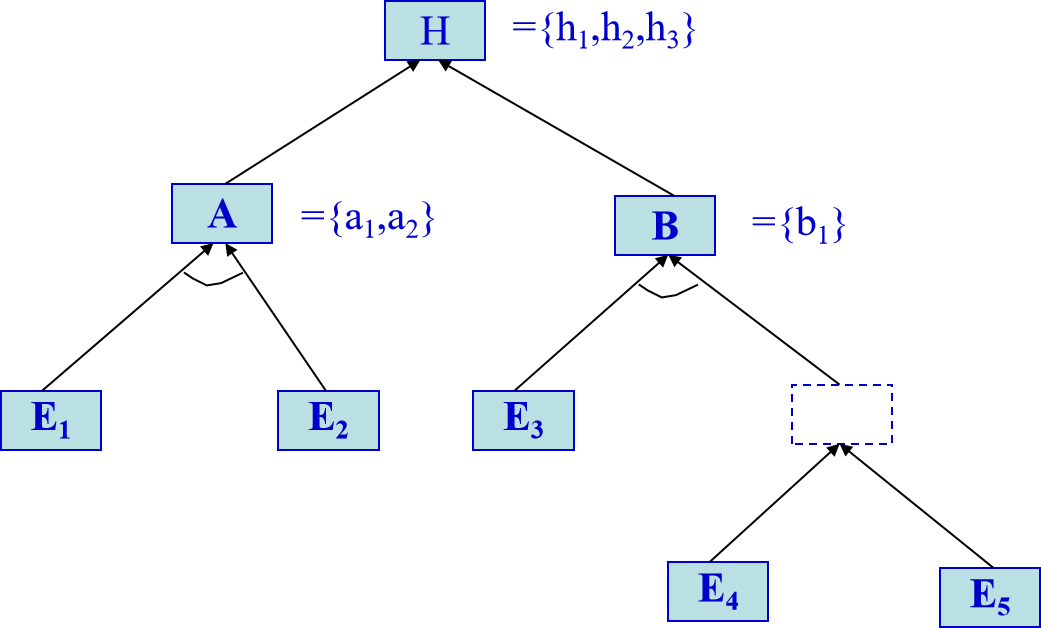
\includegraphics[width=0.6\textwidth]{AI32C42019112808.PNG}
\caption{推理网络}
\label{AI32fig2808}
\end{figure}
%%%%%%%%%%%%%%%%%%%%%%%%%%%%%%%%%%%%%%%%%%
\end{result}

(1) 求$\textup{CER}(A)$
\begin{align*}
∵ \textup{CER}(E_1\,\,  AND\,\,  E_2)&=\min\{\textup{CER}(E_1), \textup{CER}(E_2)\}=\min\{0.8,  0.6\}=0.6.\\
   m({a_1}, {a_2})&=\{0.6\times 0.3, 0.6\times 0.5\}=\{0.18, 0.3\}.\\
   \textup{Bel}(A)&=m({a_1})+m({a_2})=0.18+0.3=0.48.\\
   P_l(A)&=1-\textup{Bel}(\neg A)=1-0=1.\\
   f(A)&=\textup{Bel}(A)+|A|/|\Omega|*[P_l(A)-\textup{Bel}(A)]=0.48+2/10*[1-0.48] =0.584.\\
 ∴  \textup{CER}(A)&=MD(A/E')\times f(A)=0.584.
\end{align*}

(2) 求\textup{CER}(B)
\begin{align*}
∵ \textup{CER}(E_3 \,\, AND\,\,  (E_4\,\,  OR\,\,  E_5))&=\min\{\textup{CER}(E_3), \max\{\textup{CER}(E_4), \textup{CER}(E_5)\}\}\\
                           &=\min\{0.9, \max\{0.5, 0.7\}\}=\min\{0.9, 0.7\}=0.7. \\
 m({b_1})&=0.7\times 0.7=0.49.\\
   \textup{Bel}(B)&=m({b_1})=0.49.\\
   P_l(B)&=1-Bel(\neg B)=1-0=1.\\
   F(B)&=\textup{Bel}(B)+|B|/|\Omega|*[P_l(B)-\textup{Bel}(B)]\\
       &=0.49+1/10*[1-0.49]=0.541.\\
  ∴ \textup{CER}(B)&=MD(B/E')\times f(B)=0.541.
\end{align*}

(3) 求$\textup{CER}(H)$, 由$r_3$可得
\begin{align*}
  m_1({h_1}, {h_2}, {h_3})&=\{\textup{CER}(A)\times 0.1, \textup{CER}(A)\times 0.5, \textup{CER}(A)\times 0.3\}\\
                      &=\{0.584\times 0.1, 0.584\times 0.5, 0.584\times 0.3\}=\{0.058, 0.292, 0.175\}
\end{align*}
\begin{align*}
  m_1(\Omega)=1-[m_1({h_1})+m_1({h_2})+m_1({h_3})] =1-(0.058+0.292+0.175)=0.475.
\end{align*}
再由$r_4$可得
\begin{align*}
  m_2({h_1}, {h_2}, {h_3})&={\textup{CER}(B)\times 0.4, \textup{CER}(B)\times 0.2, \textup{CER}(B)\times 0.1}\\
        &=\{0.541\times 0.4, 0.541\times 0.2, 0.541\times 0.1\}=\{0.216, 0.108, 0.054\}\\
  m_2(\Omega) &=1-[m_2({h_1})+m_2({h_2})+m_2({h_3})]\\
              &=1-[0.216+0.108+0.054]=0.622.
\end{align*}

求正交和$m=m_1\oplus m_2$
\begin{align*}
   K&=m_1(\Omega )\times m_2(\Omega )+m_1({h1})\times m_2({h1})+m_1({h1})\times m_2(\Omega )+m_1(\Omega )\times m_2({h1})\\
    &\quad +m_1({h_2})\times m_2({h_2})+m_1({h_2})\times m_2(\Omega )+m_1(\Omega )\times m_2({h_2})\\
    &\quad +m_1({h_3})\times m_2({h_3})+m_1({h_3})\times m_2(\Omega )+m_1(\Omega )\times m_2({h_3})\\
   &=0.475\times 0.622+0.058\times 0.216+0.058\times 0.622+0.475\times 0.216\\
   &\quad +0.292\times 0.108+0.292\times 0.622+0.475\times 0.108\\
   &\quad  +0.175\times 0.054+0.175\times 0.622+0.475\times 0.054 =0.855.
 \end{align*}
\begin{align*}
m\left(h_{1}\right) &=\frac{1}{K} \times\left[m_{1}\left(\left\{h_{1}\right\}\right) \times m_{2}\left(\left\{h_{1}\right\}\right)+m_{1}
       \left(\left\{h_{1}\right\}\right) \times m_{2}(\Omega)+m_{1}(\Omega) \times m_{2}\left(\left\{h_{1}\right\}\right)\right] \\
&=\frac{1}{0.855} \times[0.058 \times 0.216+0.058 \times 0.622+0.475 \times 0.216].
\end{align*}
同理可得:
\begin{align*}
m\left(h_{2}\right) &=\frac{1}{K} \times\left[m_{1}\left(\left\{h_{2}\right\}\right) \times m_{2}\left(\left\{h_{2}\right\}\right)+m_{1}\left(\left\{h_{2}\right\}\right) \times m_{2}(\Omega)+m_{1}(\Omega) \times m_{2}\left(\left\{h_{2}\right\}\right)\right] \\ &=\frac{1}{0.855} \times[0.292 \times 0.108+0.292 \times 0.622+0.475 \times 0.108] \\
&=0.309. \\
m\left(h_{3}\right)=& \frac{1}{K} \times\left[m_{1}\left(\left\{h_{3}\right\}\right) \times m_{2}\left(\left\{h_{3}\right\}\right)+m_{1}\left(\left\{h_{3}\right\}\right) \times m_{2}(\Omega)+m_{1}(\Omega) \times m_{2}\left(\left\{h_{3}\right\}\right)\right] \\ &=\frac{1}{0.855} \times[0.175 \times 0.054+0.175 \times 0.622+0.475 \times 0.054] \\
&=0.168.
\end{align*}
\begin{align*}
  m(\Omega )=1-[m({h_1})+m({h_2})+m{(h_3)}]=1-(0.178+0.309+0.168)=0.345.
\end{align*}

再根据$m$可得
\begin{align*}
\textup{Bel}(H)&=m({h_1})+m({h_2})+m({h_3})=0.178+0.309+0.168=0.655.\\
P_l(H)&=m(\Omega)+Bel(H)=0.345+0.655=1.
\end{align*}
\begin{align*}
  \begin{aligned}
  f(H) &=\operatorname{Bel}(H)+\frac{|H|}{|\Omega|} \times[P_l(H)-\operatorname{Bel}(H)]=0.655+\frac{3}{10} \times[1-0.6555] \\
       &=0.759.\\
  \textup{CER}(H)&=MD(H/E')\times f(H)=0.759.
  \end{aligned}
\end{align*}

\textbf{优点}: 能处理由“不知道”所引起的非精确性; 并且由于辨别框(样本空间)的子集可以是多个元素的集合, 这样更有利于领域专家在不同层次上进行知识表示.

\textbf{缺点}: 要求辨别框中的元素满足互斥条件, 这在实际系统中不易实现; 并且, 需要给出的概率分配数太多, 计算比较复杂.

%%%%%%%%%%%%%%%%%%%%%%%%%%%%%%%%%%%%%%%%%
\section{模糊推理}
用自然语言中的词或句子表示的变量
%%%%%%%%%%%%%%%%%%%%%%%%%%%%%%%%%%%%%%%
\begin{example}
变量“年龄”在普通集合中为数字变量$u=[0, 150]$, 而在模糊集和中可使用语言变量, 该语言变量的取值可以是年轻、很年轻、不很年轻、老、很老、不很老等. 这些值可看作是论域$U=[0, 150]$上模糊集的集合名.
\end{example}
%%%%%%%%%%%%%%%%%%%%%%%%%%%%%%%%%%%%%%%%%
\paragraph{模糊谓词}
设$x\in U$, $F$为模糊谓词, 即$U$中的一个模糊关系, 则模糊命题可表示为
 \begin{align}
   x\,\,  \textup{is} \,\, F,
 \end{align}
其中的模糊谓词$F$可以是大、小、年轻、年老、冷、暖、长、短等.
%%%%%%%%%%%%%%%%%%%%%%%%%%%%%%%%%%%%%%%%%
\paragraph{模糊量词}
模糊逻辑中使用的模糊量词, 如极少、很少、几个、少数、多数、大多数、几乎所有等.这些模糊量词可以很方便地描述类似于下面的命题:
\begin{itemize}
\item 大多数成绩好的学生学习都很刻苦.
\item 很少有成绩好的学生特别贪玩.
\end{itemize}

模糊概率、模糊可能性和模糊真值

设$\lambda$为模糊概率, π为模糊可能性, $\tau$为模糊真值, 则对命题还可以附加概率限定、可能性限定和真值限定:
\begin{align}
  (x\,\,  \textup{is}\,\,   F) \,\,  \textup{is}\,\,   \lambda     (x\,\,   \textup{is}\,\,   F) \,\,  \textup{is} \,\, \prod     \,\,   (x \,\,  \textup{is}\,\,   F) \,\,  \textup{is} \,\,  \tau,
\end{align}
其中, $\lambda$可以是“或许”、“必须”等; π可以是“非常可能”、“很不可能”等; τ可以是“非常真”、“有些假”等.
%%%%%%%%%%%%%%%%%%%%%%%%%%%%%%%%%%%%%%%
\begin{example}
“常青很可能是年轻的”可表示为
\begin{center}
  (Age(Chang qing) is young) is likely.
\end{center}
\end{example}
%%%%%%%%%%%%%%%%%%%%%%%%%%%%%%%%%%%%%%%%%
\paragraph{模糊修饰语}
设$m$是模糊修饰语, $x$是变量, $F$谓模糊谓词, 则模糊命题可表示为$x \,\, \textup{is} \,\, m_F$, 模糊修饰语也称为程度词, 常用的程度词有“很”、“非常”、“有些”、“绝对”等.

模糊修饰语的表达主要通过以下四种运算实现:

\ding{172} 求补   表示否定, 如“不”、“非”等, 其隶属函数的表示为
\begin{align*}
  \mu_{\neg F}(u)=1-\mu_{F}(u), u \in[0,1].
\end{align*}

\ding{173} 集中  表示“很”、“非常”等, 其效果是减少隶属函数的值:
\begin{align*}
 \mu_{\textup{非常}F}(u)=\mu_{F}^{2}(u), u \in[0,1].
\end{align*}

\ding{174} 扩张  表示“有些”、“稍微”等, 其效果是增加隶属函数的值:
\begin{align*}
    \mu_{\textup{有些}F}(u)=\mu_{F}^{\frac{1}{2}}(u), u \in[0,1].
\end{align*}

\ding{175} 加强对比  表示“明确”、“确定”等, 其效果是增加0.5以上隶属函数的值, 减少0.5以下隶属函数的值:
\begin{align*}
  \mu_{\textup{确实}F}(u)=\left\{
  \begin{array}{ll}
  {2 \mu_{F}^{2}(u)}, &  0 \leq \mu_{F}(u) \leq 0.5; \\
  {1-2\left(1-\mu_{F}(u)\right)^{2}}, & 0.5<\mu_{F}(u) \leq 1.
  \end{array}\right.
\end{align*}

在以上4种运算中, 集中与扩张用的较多.
%%%%%%%%%%%%%%%%%%%%%%%%%%%%%
\begin{example}
语言变量“真实性”取值“真”和“假”的隶属函数定义为:
\begin{align*}
  \mu_{\textup{真}}(u)&=u & u \in[0,1;\\
  \mu_{\textup{假}}(u)&=1-u & u \in[0,1].
\end{align*}
则“非常真”、“有些真”、“非常假”、“有些假”可定义为
\begin{align*}
   \mu_{\textup{非常真}}(u)=u^{2}, u \in[0,1];&\quad \mu_{\textup{非常假}}((u)=(1-u)^{2}, u \in[0,1];\\
   \mu_{\textup{有些真}}(u)=u^{\frac{1}{2}}, u \in[0,1];&\quad \mu_{\textup{有些假}}(u)=(1-u)^{\frac{1}{2}}, u \in[0,1].
\end{align*}  
\end{example}

在扎德的推理模型中, 产生式规则的表示形式是
\begin{align*}
  \textup{IF}\,\,  x \,\,   \textup{is} \,\,   F \,\,   \textup{THEN} \,\,   y \,\,   \textup{is} \,\,   G,
\end{align*}
其中$x$和$y$是变量, 表示对象; $F$和$G$分别是论域$U$和$V$上的模糊集, 表示概念.
%%%%%%%%%%%%%%%%%%%%%%%%%%%%%%%%%%%%%%%%%%%%%%%%%
\subsection{模糊概念的匹配}
语义距离用于刻划两个模糊概念之间的差异.这里主要讨论海明距离.

\textbf{离散论域}: 设$U={u_1, u_2, \cdots, u_n}$是一个离散有限论域, $F$和$G$分别是论域$U$上的两个模糊概念的模糊集, 则$F$和$G$的海明距离定义为
\begin{align}
  d(F, G)=\frac{1}{n} \times \sum_{i=1}^{n}\left|\mu_{F}\left(u_{i}\right)-\mu_{G}\left(u_{i}\right)\right|.
\end{align}

\textbf{连续论域}: 如果论域$U$是实数域上的某个闭区间$[a, b]$, 则海明距离为
\begin{align}
  d(F, G)=\frac{1}{b-a} \int_{a}^{b}\left|\mu_{F}(u)-\mu_{G}(u)\right| d(u).
\end{align}
%%%%%%%%%%%%%%%%%%%%%%%%%%%%%%%%%%%%%%%
\begin{example}
设论域$U=\{-10, 0, 10, 20, 30\}$表示温度, 模糊集
\begin{align}
  F&= 0.8/-10+0.5/0+0.1/10;\\
  G&=0.9/-10+0.6/0+0.2/10.
\end{align}
分别表示“冷”和“比较冷”, 则
\begin{align}
  d(F,G)=0.2\times (|0.8-0.9|+|0.5-0.6|+|0.1-0.2|)=0.2\times 0.3=0.06,
\end{align}
即$F$和$G$的海明距离为0.06.
\end{example}

设$F$和$G$分别是论域 $U={u_1, u_2, \cdots, u_n}$上的两个模糊概念的模糊集, 则它们的贴近度定义为
\begin{align}
  (F, G)=\frac 1 2( F\cdot G+(1-F\odot G)),
\end{align}
其中:
\begin{align}
\begin{array}{l}
F \cdot G=\vee\left(\mu_{F}\left(u_{i}\right) \wedge \mu_{G}\left(u_{i}\right)\right);\\
F \odot G=\bigwedge_{U}\left(\mu_{F}\left(u_{i}\right) \vee \mu_{G}\left(u_{i}\right)\right).
\end{array}
\end{align}
称$F\cdot G$为内积, $F\odot G$为外积.
%%%%%%%%%%%%%%%%%%%%%%%%%%%%%%%%%%%%%%%
\begin{example}
设论域$U$及其上的模糊集$F$和$G$如上例所示, 则
\begin{align*}
F\cdot G&=0.8\wedge 0.9\vee 0.5\wedge 0.6\vee 0.1\wedge 0.2 \vee  0\wedge 0\vee  0\wedge 0=0.8\vee 0.5\vee 0.1 \vee  0 \vee  0=0.8.\\
F\odot G&= (0.8\vee 0.9)\wedge (0.5\vee 0.6)\wedge (0.1\vee 0.2) \wedge (0\vee 0) \wedge (0\vee 0)\\
        &=0.9\wedge 0.6\wedge 0.2\wedge 0\wedge 0 =0.\\
(F, G)&=0.5\times (0.8+(1-0))=0.5\times 1.8=0.9.
\end{align*}
即$F$和$G$的贴近度为0.9.
\end{example}

%%%%%%%%%%%%%%%%%%%%%%%%%%%%%%%%%%%
\subsection{模糊推理}
模糊推理实际上是按照给定的推理模式, 通过模糊集合与模糊关系的合成来实现的. 主要讨论模糊关系的构造和合成运算.

%%%%%%%%%%%%%%%%%%%%%%%%%%%%%%%%%%%
\paragraph{模糊关系的构造}
%%%%%%%%%%%%%%%%%%%%%%%%%%%%%%%%%%%
\subparagraph{\textbf{模糊关系$R_m$}}

$R_m$是由扎德提出的一种构造模糊关系的方法.设$F$和$G$分别是论域$U$和$V$上的两个模糊集, 则$R_m$定义为
\begin{align}
  R_{m}=\int_{U \times V}\left(\mu_{F}(u) \wedge \mu_{G}(v)\right) \vee\left(1-\mu_{F}(u)\right) /(u, v),
\end{align}
其中, $\times$号表示模糊集的笛卡尔乘积.
%%%%%%%%%%%%%%%%%%%%%%%%%%%%%%%%%
\begin{example}\label{AIFuzzyexamp612}
 设$U=V=\{1,2,3\}$, $F$和$G$分别是$U$和$V$上的两个模糊集, 且$F=1/1+0.6/2+0.1/3,G=0.1/1+0.6/2+1/3$, 求$U\times V$上的 $R_m$
\begin{align*}
  R_{m}=\int_{U \times V}\left(\mu_{F}(u) \wedge \mu_{G}(v)\right) \vee\left(1-\mu_{F}(u)\right) /(u, v).
\end{align*}
\end{example}
%%%%%%%%%%%%%%%%%%%%%%%%%%%%%%%%%%%%
\begin{result}
\begin{align*}
  R_{m}=\left[\begin{array}{ccc}{0.1} & {0.6} & {1} \\ {0.4} & {0.6} & {0.6} \\ {0.9} & {0.9} & {0.9}\end{array}\right].
\end{align*}
如: $R_m(2, 3) =(0.6\wedge 1)\vee (1-0.6)=0.6\vee 0.4=0.6$.
\end{result}
%%%%%%%%%%%%%%%%%%%%%%%%%%%%%%%%%%%
\subparagraph{模糊关系$R_c$}
$R_c$是由玛达尼(Mamdani)提出的一种构造模糊关系的方法.

设$F$和$G$分别是论域$U$和$V$上的两个模糊集, 则$R_c$义为
\begin{align*}
  R_{c}=\int_{U \times V}\left(\mu_{F}(u) \wedge \mu_{G}(v)\right)_{\mathcal{Q}} /(u, v).
\end{align*}
%%%%%%%%%%%%%%%%%%%%%%%%%%%%%%%%%
\begin{example}
对例\ref{AIFuzzyexamp612}所给出的模糊集
\begin{align*}
  F=1/1+0.6/2+0.1/3, G=0.1/1+0.6/2+1/3,
\end{align*}
其$R_c$为
\begin{align*}
  R_{c}=\left[\begin{array}{ccc}{0.1} & {0.6} & {1} \\ {0.1} & {0.6} & {0.6} \\ {0.1} & {0.1} & {0.1}\end{array}\right],
\end{align*}
\end{example}
如$R_{c}(3,2)=\mu_{F}\left(u_{3}\right) \wedge \mu_{G}\left(v_{2}\right)=0.1 \wedge 0.6=0.1$.
%%%%%%%%%%%%%%%%%%%%%%%%%%%%%%%%%%%
\subparagraph{模糊关系$R_g$}
$R_g$是米祖莫托(Mizumoto)提出的一种构造模糊关系的方法.

设$F$和$G$分别是论域$U$和$V$上的两个模糊集, 则$R_g$定义为
\begin{align*}
  R_{g}=\int_{U \times V}\left(\mu_{F}(u) \rightarrow \mu_{G}(v)\right) /(u, v),
\end{align*}
其中
\begin{align*}
  \mu_{F}(u) \rightarrow \mu_{G}(v)=
  \left\{
  \begin{array}{ll}
  {1}, & \mu_{F}= \mu_{F}(u) \leq \mu_{G}(v)^{\top};\\
  \mu_{F}(v), &  \mu_{F}(u)>\mu_{G}(v) ^{\top}.
  \end{array}
  \right.
\end{align*}
%%%%%%%%%%%%%%%%%%%%%%%%%%%%%%%%%
\begin{example}
对例\ref{AIFuzzyexamp612}所给出的模糊集
\begin{align*}
  F=1/1+0.6/2+0.1/3, G=0.1/1+0.6/2+1/3,
\end{align*}
其$R_g$为
\begin{align*}
  R_{g}=\left[\begin{array}{ccc}{0.1} & {0.6} & {1} \\ {0.1} & {1} & {1} \\ {1} & {1} & {1}\end{array}\right].
\end{align*}
\end{example}
%%%%%%%%%%%%%%%%%%%%%%%%%%%%%%%%%%%
\subparagraph{模糊假言推理}
\subsubsection{模糊假言推理举例}
设$F$和$G$分别是$U$和$V$上的两个模糊集, 且有知识
\begin{align*}
   \textup{知识}: &\quad\quad\textup{IF}\,\,   x \,\, is \,\, F \,\, \textup{THEN}\,\,   y\,\,  \textup{is} \,\,G.
\end{align*}

若有$U$上的一个模糊集$F'$, 且$F$可以和$F'$匹配, 则可以推出$y$  is  $G'$, 且$G'$是$V$上的一个模糊集.这种推理模式称为模糊假言推理, 其表示形式为:
\begin{align*}
   \textup{知识}: &\quad\quad\textup{IF}\,\,   x \,\, is \,\, F \,\, \textup{THEN}\,\,   y\,\,  \textup{is} \,\,G\\
   \textup{证据}: &\quad\quad\textup{IF}\,\,   x \,\, is \,\, F'\\
   &--------------\\
  \textup{结论}:  &\qquad\qquad\qquad \textup{THEN}\,\,   y\,\,  \textup{is} \,\,G'
\end{align*}
在这种推理模式下, 模糊知识
\begin{align*}
   &\textup{IF}\,\,   x \,\, is \,\, F \,\, \textup{THEN}\,\,   y\,\,  \textup{is} \,\,G,
\end{align*}
表示在$F$与$G$之间存在着确定的因果关系, 设此因果关系为$R$. 则有
\begin{align*}
  G'=F'\circ R,
\end{align*}
其中的模糊关系$R$, 可以是$R_m$、$R_c$或$R_g$中的任何一种.
%%%%%%%%%%%%%%%%%%%%%%%%%%%%%%%%%%%
\paragraph{模糊推理的基本方法}
%%%%%%%%%%%%%%%%%%%%%%%%%%%%%%%%%
\begin{example}
  对例4.19所给出的$F$、$G$, 以及所求出的$R_m$, 设有已知事实: $\{x\, \textup{is}\, \textup{较小}\}$, 并设“较小”的模糊集为: 较小=1/1+0.7/2+0.2/3, 求在此已知事实下的模糊结论.
\end{example}
%%%%%%%%%%%%%%%%%%%%%%%%%%%%%%%%%%%%
\begin{result}
本例的模糊关系$R_m$已在例6.12中求出, 设已知模糊事实“较小”为$F'$, $F'$与$R_m$的合成即为所求结论$G'$.
\begin{align*}
G^{\prime}=F^{\prime} \circ R_{m}=\{1,0.7,0.2\} \circ
\left[
\begin{array}{ccc}
{0.1} & {0.6} & {1} \\
{0.4} & {0.6} & {0.6} \\
 {0.9} & {0.9} & {0.9}\end{array}\right]
=\{0.4, 0.6,1\},
\end{align*}
即所求出的模糊结论$G'$为 $G'=0.4/1+0.6/2+1/3$.
\end{result}
%%%%%%%%%%%%%%%%%%%%%%%%%%%%%%%%%%%
\subparagraph{模糊拒取式推理}
设$F$和$G$分别是$U$和$V$上的两个模糊集, 且有知识
\begin{align*}
  \textup{IF}\,\,   x \,\, is \,\, F \,\, \textup{THEN}\,\,   y\,\,  \textup{is} \,\, G
\end{align*}

若有$V$上的一个模糊集$G'$, 且$G$可以和$G'$匹配, 则可以推出$x\,\,\textup{is} \,\,  F'$, 且$F'$是$U$上的一个模糊集.这种推理模式称为\textbf{模糊拒取式推理}, 其表示形式为:
\begin{align*}
   \textup{知识}: &\quad\quad\textup{IF}\,\,   x \,\, is \,\, F \,\, \textup{THEN}\,\,   y\,\,  \textup{is} \,\,G\\
   \textup{证据}: &\qquad\qquad\qquad\,\, \textup{THEN}\,\,   z\,\,  \textup{is} \,\,H\\
   &--------------\\
  \textup{结论}:  &\quad\quad\textup{IF}\,\,   x \,\, is \,\, F'.
\end{align*}
在这种推理模式下, 模糊知识
\begin{align*}
  \textup{IF}\,\,   x \,\, is \,\, F \,\, \textup{THEN}\,\,   y\,\,  \textup{is} \,\, G;
\end{align*}
也表示在$F$与$G$之间存在着确定的因果关系, 设此因果关系为$R$, 则有
\begin{align*}
  F'=R\circ G',
\end{align*}
其中的模糊关系$R$, 可以是$R_m$、$R_c$或$R_g$中的任何一种.

%%%%%%%%%%%%%%%%%%%%%%%%%%%%%%%%%
\begin{example}
  设$F$和$G$如例4.19所示, 已知事实为$\{y \,\,\textup{ is\,\,  较大}\}$且“较大”的模糊集为: 较大$=0.2/1+0.7/2+1/3$, 若已知事实与$G$匹配, 以模糊关系$R_c$为例, 在此已知事实下推出$F'$.
\end{example}
%%%%%%%%%%%%%%%%%%%%%%%%%%%%%%%%%%%%
\begin{result}
本例的模糊关系$R_c$已在前面求出, 设模糊概念“较大”为$G'$, 则$R_c$与$G'$的合成即为所求的$F'$.
\begin{align*}
  F^{\prime}=R_{c} \circ G^{\prime}=
  \left[
  \begin{array}{ccc}
  {0.1} & {0.6} & {1} \\
  {0.1} & {0.6} & {0.6} \\
  {0.1} & {0.1} & {0.1}\end{array}\right]
  \circ\left[
  \begin{array}{c}
  {0.2} \\
   {0.7} \\
    {1}\end{array}
    \right]
 =\left[\begin{array}{c}
 {1} \\ {0.6} \\ {0.1}
 \end{array}
  \right],
\end{align*}
即所求出的$F'$为 $ G'=1/1+0.6/2+0.1/3$.
\end{result}
%%%%%%%%%%%%%%%%%%%%%%%%%%%%%%%%%%%
\subparagraph{模糊假言三段论推理}
设$F,G,H$分别是$U,V,W$上的3个模糊集, 且由知识
\begin{align*}
   &\textup{IF}\,\,   x \,\, is \,\, F \,\, \textup{THEN}\,\,   y\,\,  \textup{is} \,\,G\\
   &\textup{IF}\,\,   y \,\, is \,\, G \,\, \textup{THEN}\,\,   z\,\,  \textup{is} \,\,H
\end{align*}
则可推出:
\begin{align*}
   \textup{IF}\,\,   x \,\, is \,\, F \,\,\textup{THEN}\,\,   z\,\,  \textup{is} \,\,H.
\end{align*}

 这种推理模式称为\textbf{模糊假言三段论推理}. 它可表示为:
\begin{align*}
   &\textup{IF}\,\,   x \,\, is \,\, F \,\, \textup{THEN}\,\,   y\,\,  \textup{is} \,\,G\\
   &\textup{IF}\,\,   y \,\, is \,\, G \,\, \textup{THEN}\,\,   z\,\,  \textup{is} \,\,H\\
   &------------\\
   &\textup{IF}\,\,   x \,\, is \,\, F \,\, \textup{THEN}\,\,   z\,\,  \textup{is} \,\,H\\
\end{align*}

在模糊假言三段论推理模式下, 模糊知识
\begin{align*}
   r_1:  \textup{IF}\,\,   x \,\, is \,\, F \,\, \textup{THEN}\,\,   y\,\,  \textup{is} \,\,G,
\end{align*}
表示在$F$与$G$之间存在着确定的因果关系, 设此因果关系为$R_1$.

模糊知识
\begin{align*}
   r_2:  \textup{IF}\,\,   y \,\, is \,\, G \,\, \textup{THEN}\,\,   z\,\,  \textup{is} \,\, H,
\end{align*}
表示在$G$与$H$之间存在着确定的因果关系, 设此因果关系为$R_2$.

 若模糊假言三段论成立, 则模糊结论
\begin{align*}
  r_3:  \textup{IF}\,\,   x \,\, is \,\, F \,\, \textup{THEN}\,\,   z\,\,  \textup{is} \,\, H
\end{align*}
的模糊关系$R_3$可由$R_1$与$R_2$的合成得到. 即
\begin{align*}
  R_3=R_1\circ R_2.
\end{align*}
这里的关系$R_1$、$R_2$和$R_3$都可以是前面所讨论过的$R_m$、$R_c$、$R_g$中的任何一种.

%%%%%%%%%%%%%%%%%%%%%%%%%%%%%%%%%
\begin{example}
  设$U=W=V={1, 2, 3}$, $E=1/1+0.6/2+0.2/3$, $F=0.8/1+0.5+0.1/3, G=0.2/1+0.6+1/3$.按$R_g$求$E\times F\times G$上的关系$R$.
\end{example}
%%%%%%%%%%%%%%%%%%%%%%%%%%%%%%%%%%%%
\begin{result}
先求$E\times F$上的关系$R_1$
\begin{align*}
  R_{1}=\left[\begin{array}{ccc}{0.8} & {0.5} & {0.1} \\ {1} & {0.5} & {0.1} \\ {1} & {1} & {0.1}\end{array}\right].
\end{align*}

再求$E\times G$上的关系$R_2$
\begin{align*}
  R_{2}=\left[\begin{array}{ccc}{0.2} & {0.6} & {1} \\ {0.2} & {1} & {1} \\ {1} & {1} & {1}\end{array}\right].
\end{align*}

最后求$E\times F\times G$上的关系$R$
\begin{align*}
  R=R_{1} \circ R_{2}=\left[\begin{array}{ccc}{0.2} & {0.6} & {0.8} \\ {0.2} & {0.6} & {1} \\ {0.2} & {1} & {1}\end{array}\right].
\end{align*}
\end{result}
%%%%%%%%%%%%%%%%%%%%%%%%%%%%%%%%%%%%%%%%%%
\section{高阶模糊推理}
\section{作业}
%%%%%%%%%%%%%%%%%%%%%%%%%%%%%%%%%%%%%%%%%%%%%%%%
\begin{think}
 设有如下一组推理规则:
\begin{Verbatim}
    r1:  IF  E1  THEN  E2 (0.6)
    r2:  IF  E2  AND  E3  THEN  E4 (0.7)
    r3:  IF  E4  THEN  H (0.8)
    r4:  IF  E5  THEN  H (0.9)
\end{Verbatim}
且已知$CF(E1)=0.5$,  $CF(E2)=0.6$,  $CF(E3)=0.7$.求$CF(H)=?$
\end{think}
%%%%%%%%%%%%%%%%%%%%%%%%%%%%%%%%%%%%%%%%%%%%%%%%
\begin{think}
设$ U=V=\{1, 2, 3, 4, 5\}$且有如下推理规则:
$$\textup{IF} \,  x  \, \textup{is} \,  \textup{少}\,   \textup{THEN} \,  y  \, \textup{is}\,  \textup{多}$$
其中, “少”与“多”分别是$U$与$V$上的模糊集, 设
\begin{align}
  \textup{少}&=0.9/1+0.7/2+0.4/3\\
  \textup{多}&=0.3/3+0.7/4+0.9/5
\end{align}
已知事实为
\begin{align}
  x\,\,  \textup{is}\,\,  \textup{较少}
\end{align}
“较少”的模糊集为
\begin{align}
  \textup{较少}=0.8/1+0.5/2+0.2/3
\end{align}
请用模糊关系$R_m$求出模糊结论.
\end{think}
%%%%%%%%%%%%%%%%%%%%%%%%%%%%%%%%%%%
